Para realizar el experimento, debe ejecutar el archivo datasets.py y este le generara los 6 datasets(en caso de error al ejecutar, ejecutar nuevamente hasta que funcione), luego simplemente debe ejecutar el archivo main.cpp, este le generar un archivo csv con los tiempos de ejecucion, estos datos se deben pasas a un excel para generar los gráficos. Cabe recalcar que los costos calculados se imprimen directamente en la terminal una vez es ejecutado el main. Si desea cambiar los costos de cada operación, debe modificar los archivos txt que contienen los costos de cada operación(cost$\_$insert.txt, cost$\_$delete.txt, cost$\_$replace.txt, cost$\_$transpose.txt).
Los resultados de tiempo obtenidos escritos en el archivo csv, igual que los códigos y archivos datasets creados se pueden encontrar en el siguiente enlace:\\
\url{https://github.com/FrancoSepulveda-USM/Algoritmos-y-complejidad/tree/main/Tarea2_y_3}

A continuación, se presentan los gráficos generados para los diferentes conjuntos de datos utilizados en la experimentación, para estos se uso como eje x el máximo largo entre las dos cadenas, mientras que el eje y corresponde al tiempo de ejecución.

\begin{enumerate}
    \item \textbf{Dataset1}: 
    \begin{figure}[H]
        \centering
        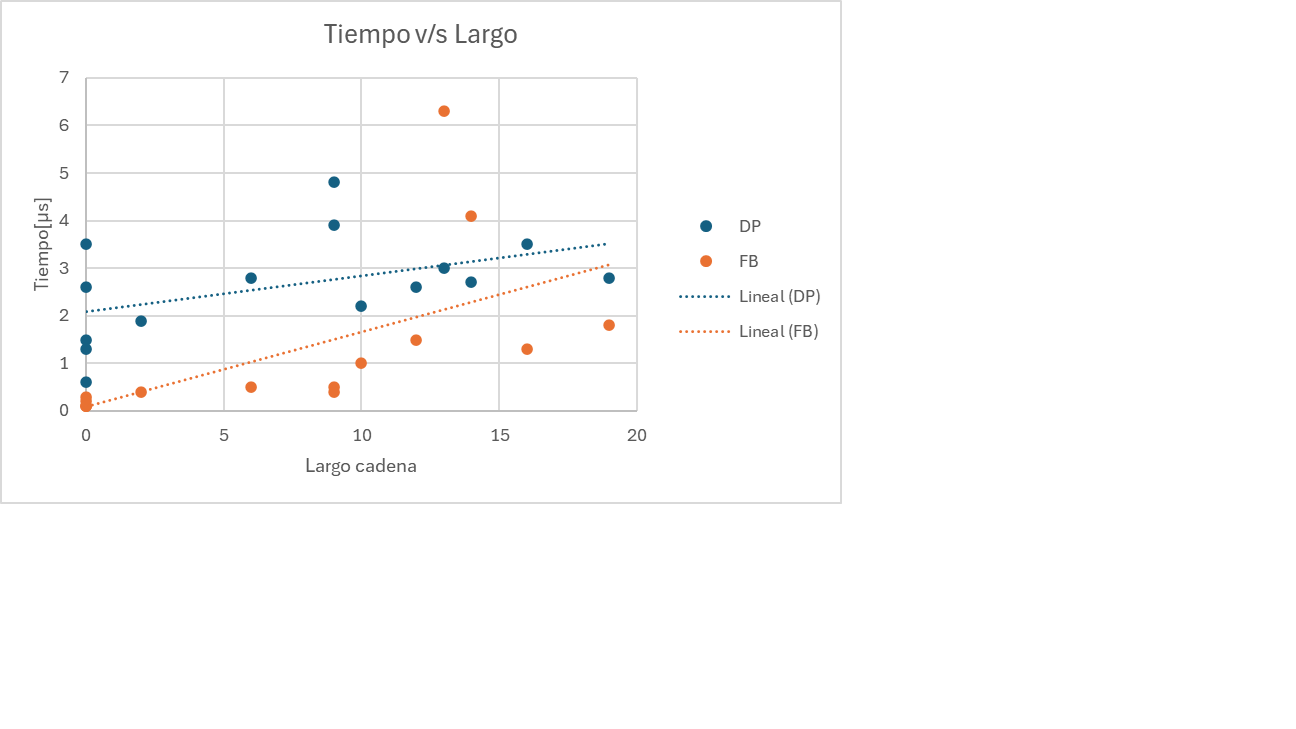
\includegraphics[width=\textwidth]{tikz/Grafico1.png}
        \caption{Gráfico correspondiente a Dataset1 con cadenas vacías.}
        \label{fig:dataset1}
    \end{figure}

    \item \textbf{Dataset2}: 
    \begin{figure}[H]
        \centering
        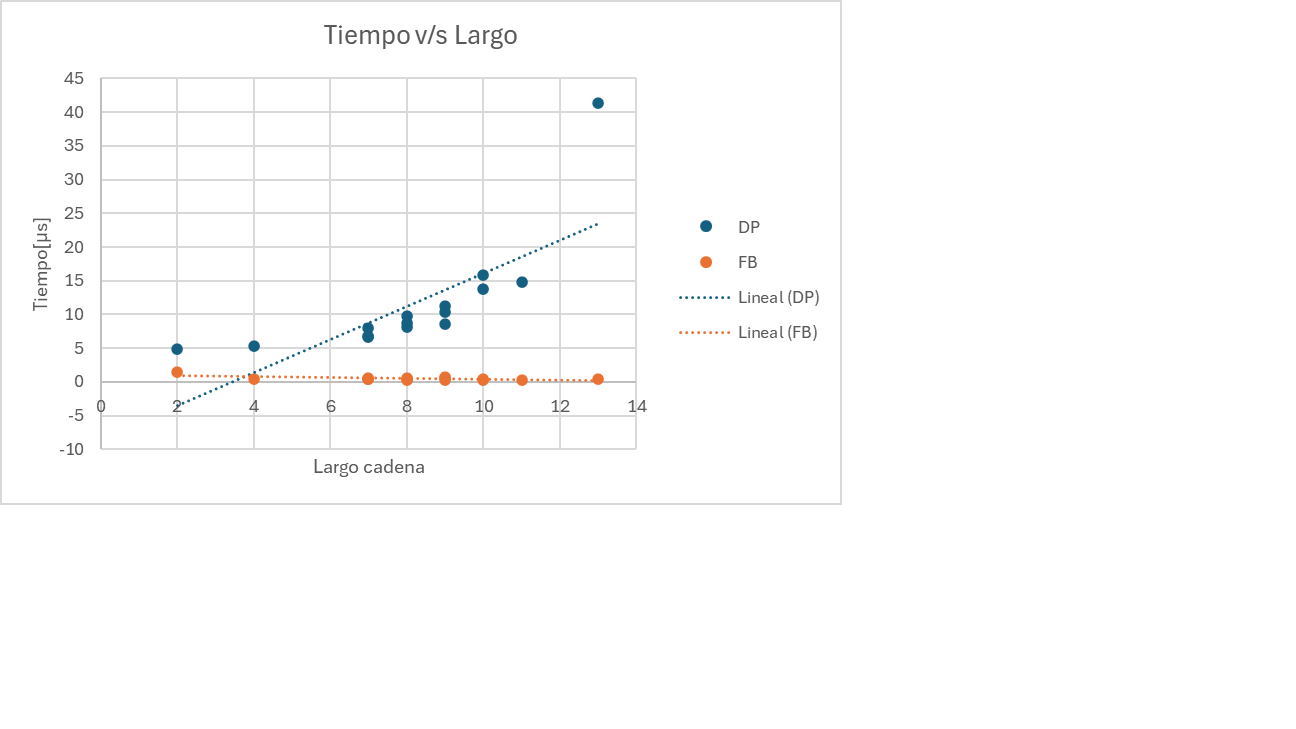
\includegraphics[width=\textwidth]{tikz/Grafico2.png}
        \caption{Gráfico correspondiente a Dataset2 con cadenas identicas.}
        \label{fig:dataset2}
    \end{figure}

    \item \textbf{Dataset3}: 
    \begin{figure}[H]
        \centering
        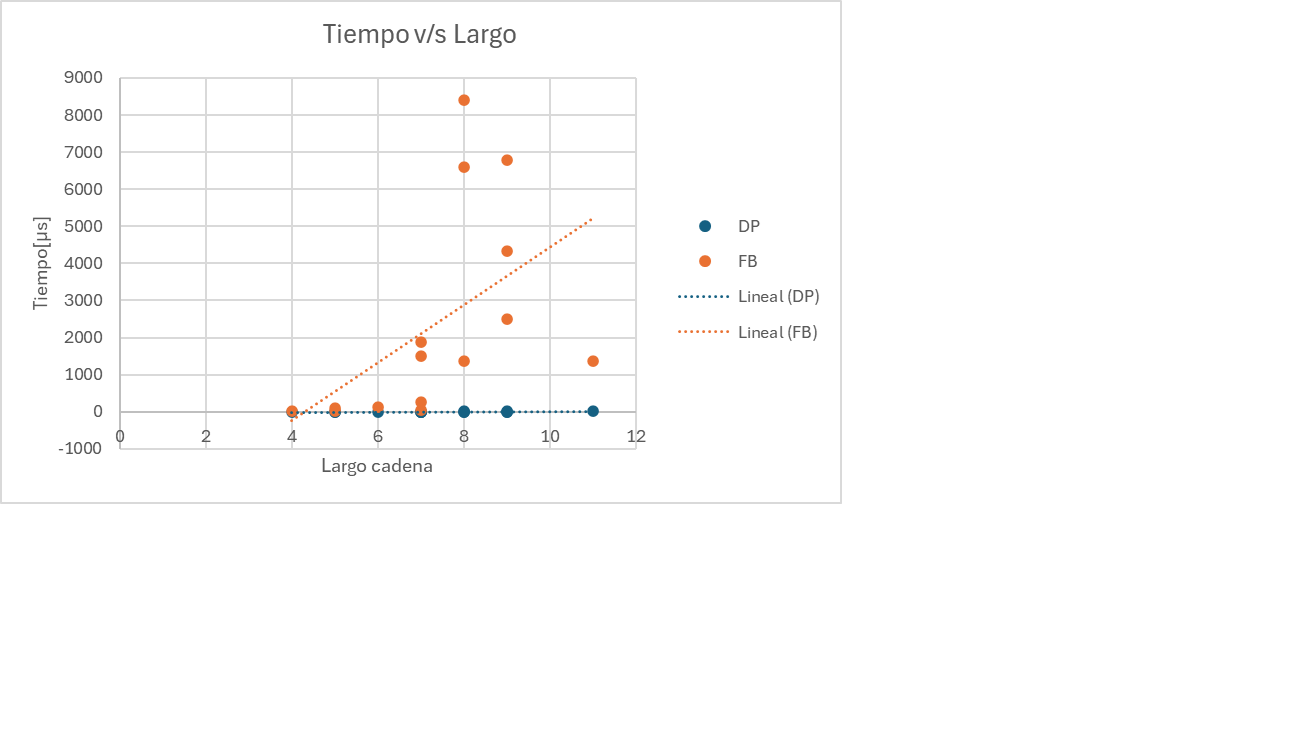
\includegraphics[width=\textwidth]{tikz/Grafico3.png}
        \caption{Gráfico correspondiente a Dataset3. Cadenas con caracteres repetidos.}
        \label{fig:dataset3}
    \end{figure}

    \item \textbf{Dataset4}: 
    \begin{figure}[H]
        \centering
        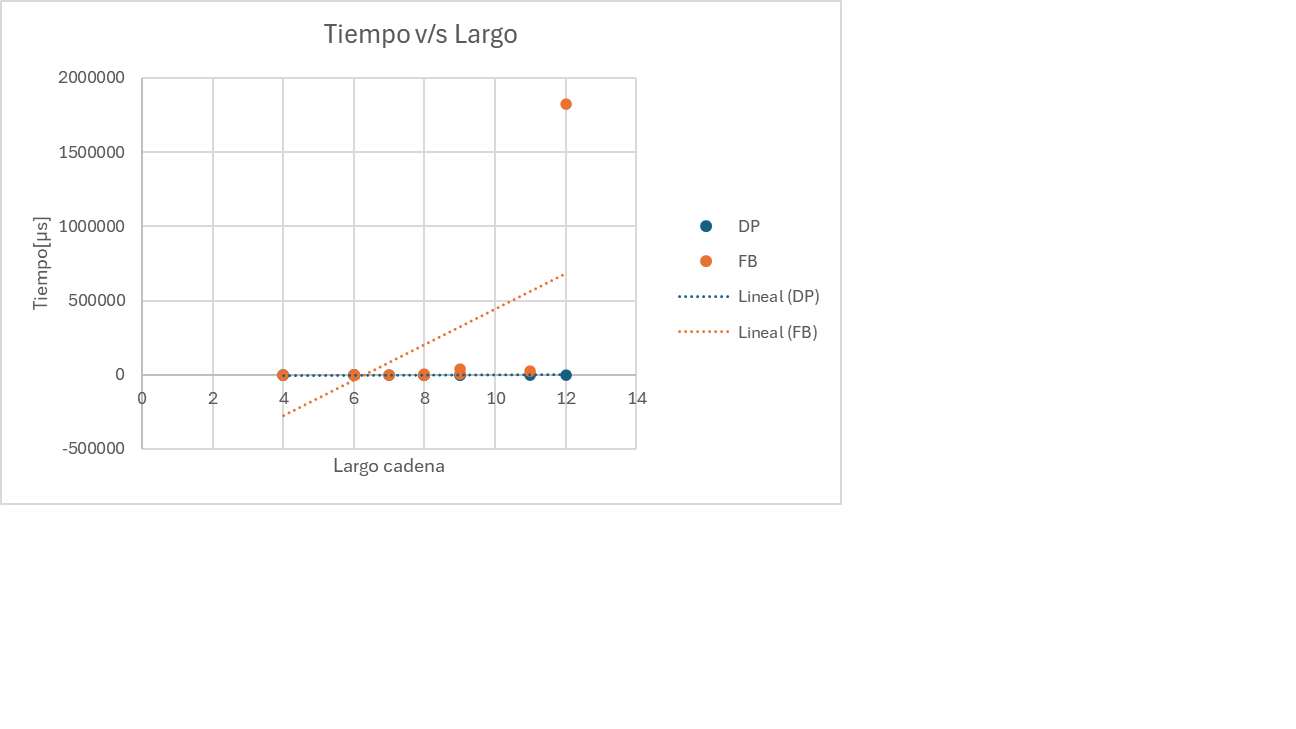
\includegraphics[width=\textwidth]{tikz/Grafico4.png}
        \caption{Gráfico correspondiente a Dataset4 con cadenas aleatorias de mismo tamaño.}
        \label{fig:dataset4}
    \end{figure}

    \item \textbf{Dataset5}: 
    \begin{figure}[H]
        \centering
        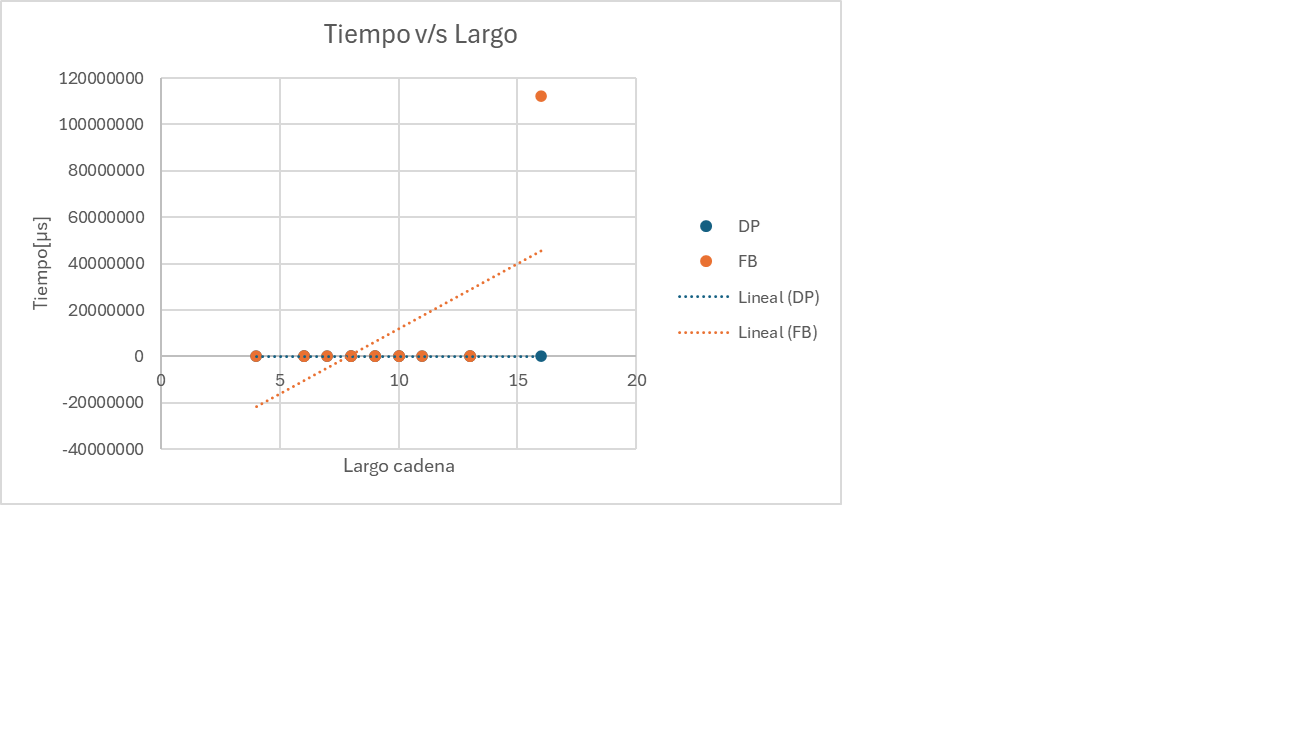
\includegraphics[width=\textwidth]{tikz/Grafico5.png}
        \caption{Gráfico correspondiente a Dataset5 con cadenas aleatorias de diferentes tamaños.}
        \label{fig:dataset5}
    \end{figure}

    \item \textbf{Dataset6}: 
    \begin{figure}[H]
        \centering
        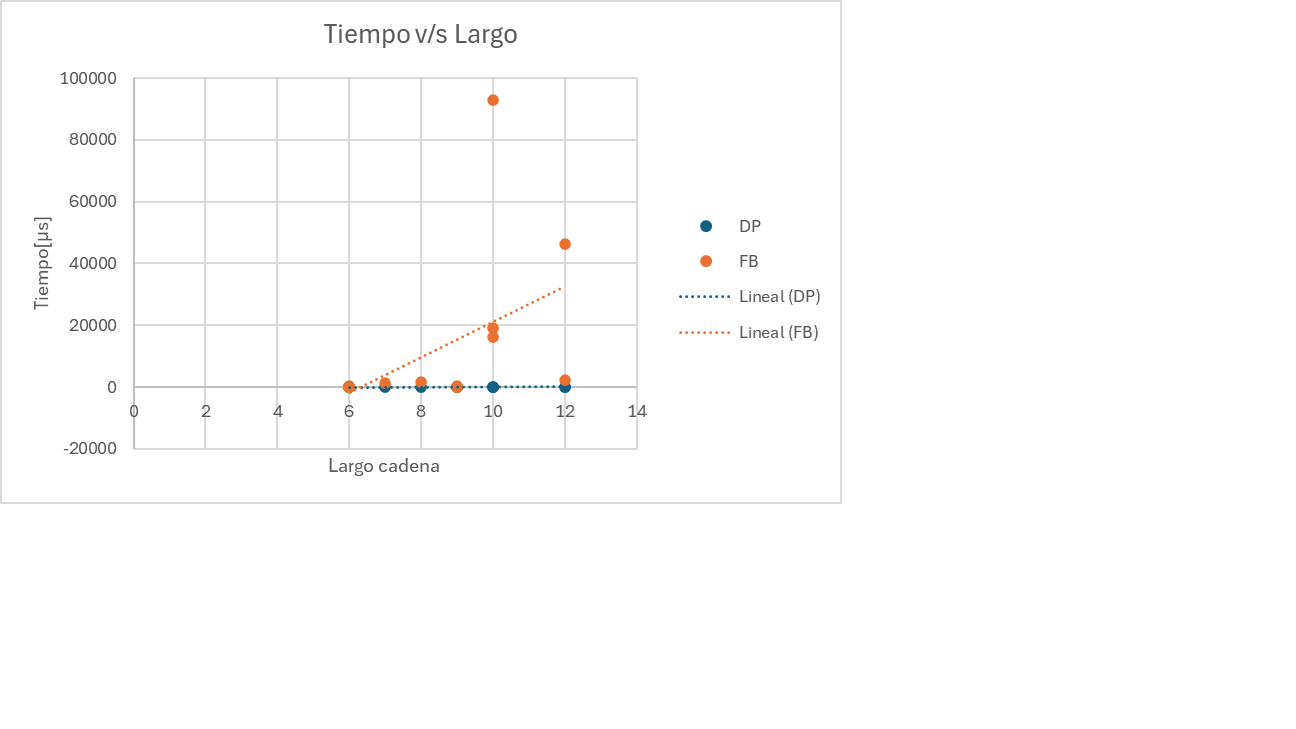
\includegraphics[width=\textwidth]{tikz/Grafico6.png}
        \caption{Gráfico correspondiente a Dataset6. Cadenas con transposiciones.}
        \label{fig:dataset6}
    \end{figure}
\end{enumerate}
